\documentclass[a4paper, twoside, 11pt]{article}
\usepackage[margin=1.5cm]{geometry}
\usepackage[]{xcolor}
\usepackage{cite}
\usepackage{graphicx}
\usepackage{listings}
\usepackage{float}
\usepackage{amsmath}
% define the title
\author{L. ~Towell, L.M.Towell@liverpool.ac.uk}

%defines the title
\title{Assignment 4:\break OpenMP \& MPI Hybrid implementation of the N body problem.}

\begin{document}
	%generate the title
	\maketitle

\maketitle
\section{The processing of Compiler reports and Code Profiling}
Initial compilation of the serial code using the intel compiler was performed using the command `icc serialCode.c -qopt-report3 -O2` this produced an optrpt file which outlines the tasks that the compiler has performed in order to optimise the code base.

From this file I am then able to see that the compiler has made various changes to the loops within the main function. These changes include vectorisation to multiple loops including the loop for working out new locations and the loops for initialising the variables in the testInit() function.

Throughout the output report the compiler has highlighted that its changes should have resulted in the potential speedup of functions. \textit{Figure 1} below are the results of comparing the serialCode with no optimisations and using the intel compiler with -O2 optimisation.

\begin{figure}[H]
	\centering
	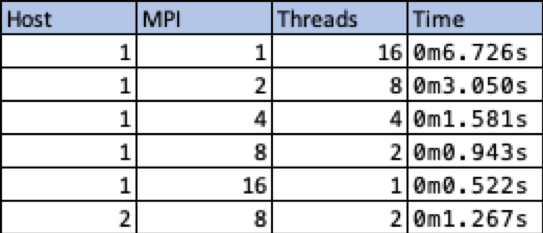
\includegraphics[scale=0.6]{images/timings}
	\caption{Hotspot Analysis of the Serial Code}
\end{figure}

As well as compiler optimisation I have also made use of sections to identify the specific parts of the code that where taking the most time to run. I have profiled the code at the beginning of the project using the Intel VTune application to view and analyse the code hotspots when running the program. \textit{Figure 2} and \textit{Figure 3} shows the hotspots of the code base and as you can see the main function is taking the most time to run.
\begin{figure}[H]
	\centering
	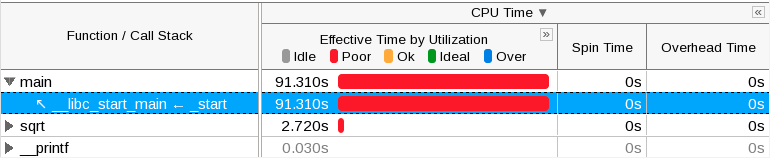
\includegraphics[scale=0.5]{images/profile1}
	\caption{Hotspot Analysis of the Serial Code}
\end{figure}
\begin{figure}[H]
\centering
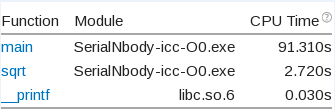
\includegraphics[scale=0.5]{images/profile2}
\caption{Timing Summary of Functions}
\end{figure}
\section{Parallelisation strategy }

As is mentioned in section 2 the section highlights that 90\% of the computation time is spent in the main function, for this reason I decided to focus my efforts on the main function.
When parallelising the code base I have decided to use a mixture of MPI and OpenMP.
The MPI that I have used includes the MPI\_Bcast function and the MPI\_Allgather functions. I have made use of the broadcast function in order to distribute the global variables across the MPI processes. I have then made use of the MPI\_Allgather function at the end of each timestamp to gather the new positions of each body. This allows the root node to refresh the X and Y values for each body and then update the value of the x and y array on each node.

Within the code base I have also made use of OpenMP. The OpenMP that I have used is two "\#pragma omp parallel for" loops. The first for loop is for calculating the position and vleocities of the bodies. The second OMP for loop is then used for updating the x and y values of each body. The x and y variables that are updated are stored within local versions of the variables and these are then gathered in using an MPI\_Allgather function as described above.

\section{Serial Code Vs MPI \& OpenMP Code}
I have ran the code on several different combinations of Hosts, MPI nodes and OpenMP threads, \textit{Figure 4} shows my findings from running the code using the script that was provided. The code that is marked in red differs text is where the accuracy of the results diminishes. If I had more time to complete this assignment one of the improvements would be to look into the reason for this discrepancy. I have assessed the accuracy of my code by comparing the answers that I achieve from the parallel code against the answers that are returned from the serial code I was provided. 

\begin{figure}[H]
	\centering
	
\includegraphics[scale=0.6]{images/compilerTimings}
	\caption{Comparison of Compiler Timings}
\end{figure}
 
 The most accurate and fastest combination of Hosts, MPI processes and threads that I have found is running on 1 host with 8 MPI processes and 2 threads per MPI process which produced a time of 0.943 seconds. I did look into trying with 2 hosts 8 MPI processes and 2 threads per node however this did not result in a beneficial speedup I believe the reason for this is because of the management of memory between hosts having a negative effect. The optimum solution produces a speedup of 83.74 compared to the serial code timings shown in \textit{Figure 4}.
 
\section{Scaling of the Code to Model Galaxy Formation}
In order to model the universe one of the requirements is going to be the ability to cope with the massive amounts of data which would be generated because of the need to analyse and calculate the position of around 100 billion bodies. To do this you are going to need to make use of large amounts of memory. The mapping of 100 billion bodies would require a massive amount of computation which would mean that you would need a large amount of data to be processed at the same time. In this assignment I have made use of MPI/OpenMP hybrid paralellisation however to map the galaxy because I would be working out the location and velocity for billions of bodies I would look into how to parallelise the calculations using OpenMP and GPU devices .

The use of GPUs would mean I can attempt to break the parellization of the 100 billion bodies across multiple threads which are connected to multiple GPUs which would then enable me to make use of OMP threads and CUDA threads to hopefully produce and optimum result. I believe that the breakdown of the code would be very similar however I would additionally parallelise the initialisation of variables as for 100 billion objects this would become very time intensive. I would also pay more attention to memory allocation.
\end{document}
